\documentclass{article}
\usepackage{isotope}
\usepackage{amsmath}
\usepackage{graphicx}
\usepackage{float}

\title{NE 770 Homework 1}
\author{William Dawn}

\begin{document}

\maketitle

\begin{enumerate}
  \item Evaluate the integral
    \begin{equation} \label{eq:p1}
        \int_0^{\pi} \theta \sin(\theta) \; d\theta
    \end{equation}
    by Monte Carlo. Report and plot the mean, the variance, and uncertainty in
    the mean as a function of number of samples. Compare to the analytic 
    solution.

    The anti-derivative can be evaluated using an integral table and the exact
    value of the integral calculated.
    \begin{align}
      \int_0^{\pi} \theta \sin(\theta) \; d\theta &= \left. - \theta
        \cos(\theta) + \sin(\theta) \right\rvert_0^{\pi} \\
      &= (- \pi (-1) + 0) - 0 \\
      &= \pi
    \end{align}

    Equation \eqref{eq:p1} can be approximated as a sum.
    \begin{align}
      \int_0^{\pi} \theta \sin(\theta) \; d\theta &= 
        \int_0^{\pi} \left( \pi \theta \sin(\theta) \right) \left(
        \frac{d\theta}{\pi} \right) \\
      &= \frac{1}{N} \sum_{i=1}^{N} \left( \pi \theta_i \sin(\theta_i) \right)
    \end{align}
    Where $\theta_i$ is uniformly distributed on the interval $[0,\pi]$.
    Statistical quantities of interest are then calculated as follows.
    \begin{align}
      z(\theta) &= \theta \sin(\theta) \\
      \hat{z} &= \frac{1}{N} \sum_{i=1}^{N} z(\theta_i) \\
      \hat{\sigma}^2 &= \left( \frac{1}{N} \sum_{i=1}^{N} z(\theta_i)^2 \right)
        - \hat{z} \\
      \hat{\sigma}^2_{\hat{z}} &= \frac{\hat{\sigma}^2}{N}
    \end{align}
    These quantities are tabulated for each sampling iteration $i$ for $i = 1
    \ldots 10^3$ and plotted. The mean approaches the expected value ($\pi$) the
    variance approaches approximately 3.7 and the uncertainty in the mean
    approaches zero by the expected $\frac{1}{N}$ relation.

    \begin{figure}[H]
      \centering
      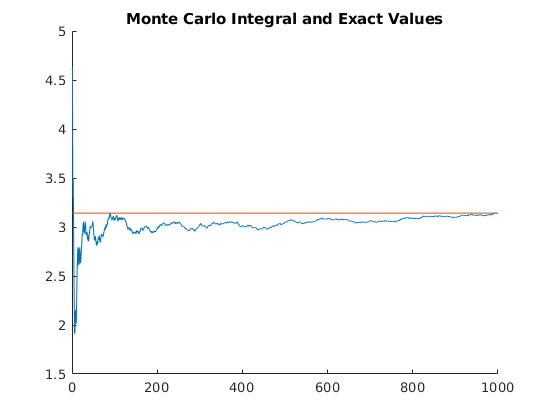
\includegraphics[width=0.8\textwidth]{integral}
      \caption{Mean of the function approaching the exact value.}
      \label{fig:integral}
    \end{figure}
    \begin{figure}[H]
      \centering
      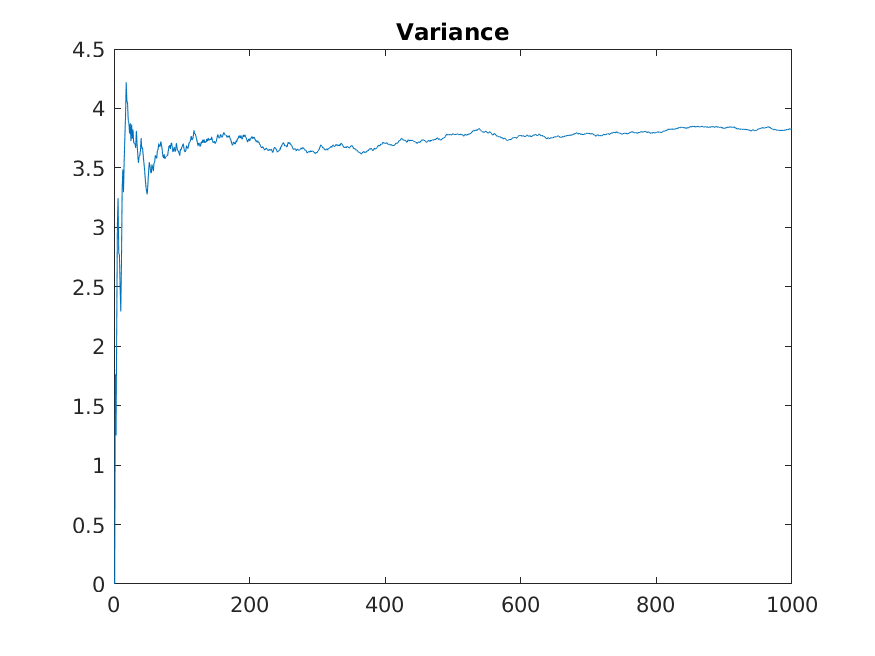
\includegraphics[width=0.8\textwidth]{variance}
      \caption{Variance of the function approaching a constant value.}
      \label{fig:variance}
    \end{figure}
    \begin{figure}[H]
      \centering
      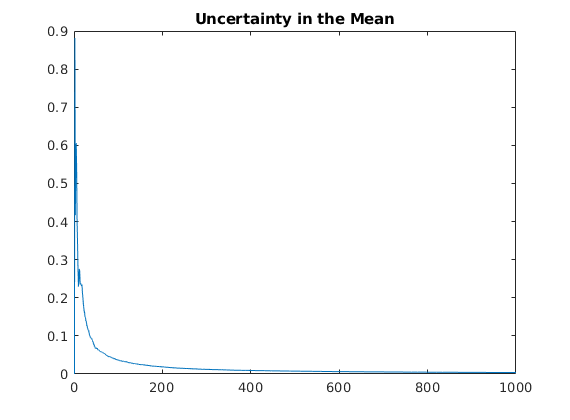
\includegraphics[width=0.8\textwidth]{uncertainty}
      \caption{Uncertainty in the mean approaching zero.}
      \label{fig:uncertainty}
    \end{figure}

  \item A common expression for the fission neutron spectrum is 
    \begin{equation}
      \chi(E) = 0.453 \exp(-E/0.965) \sinh\left(\sqrt{2.29E}\right)
    \end{equation}
    where $E \in [0,\infty)$ is in MeV. Note $\chi(E)$ is a PDF on the
    interval. The average number of neutrons emitted in fussion from 
    \isotope[235]{U} as a function of energy can be taken to be
    \begin{equation}
      \nu(E) = 
      \begin{cases}
        2.42 + 0.066 E & E \le 1 \\
        2.349 + 0.15 E & E >   1
      \end{cases}
    \end{equation}
    \begin{enumerate}
      \item Show numerically that the standard rejection scheme generates
        energies distributed according to the fission neutron spectrum. Verify
        numerically the efficency of the rejection scheme.

        Numerical sampling requires a finite domain. For the purposes of this
        investigation, energy is bounded at an upper limit of 20 MeV noting
        $\chi(20 \text{MeV}) \approx 10^{-7}$. 
        The sampling of the rejection scheme implemented for $10^6$ samples is
        given in Figure \ref{fig:standard_rejection}. Analytically the
        efficiency of the standard rejection scheme is given.
        \begin{equation} \label{eq:standard_efficiency}
          \epsilon = \frac{1}{h_{max} (b-a)}
        \end{equation}
        Where $b$ is the upper sampling bound and $a$ is the lower sampling
        bound. For maximum efficincy of the standard rejecstion scheme,
        $h_{max}$ is chosen as the maximum of the function in the sampling
        domain. It was determined that numerically, it was determined that
        \begin{equation}
          h_{max} = \max_{E \in [0,20]} \chi(E) = 0.358136317809776
        \end{equation}
        Then, the analytic efficiency is 0.139612. The observed efficiency of
        this scheme as implemented numerically for $10^6$ samples was 0.139837.

        \begin{figure}
          \centering
          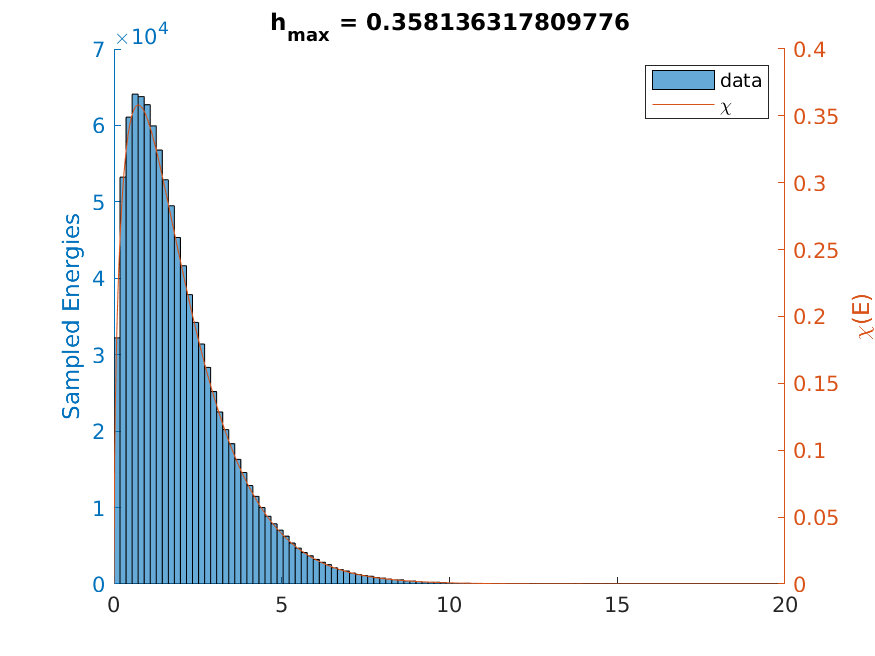
\includegraphics[width=0.8\textwidth]{standard_rejection}
          \caption{Sampling with standard rejection and maximum efficiency.}
          \label{fig:standard_rejection}
        \end{figure}

      \item Verify numerically that increasing the $h_{max}$ value for the
        rejection scheme still generates energies distributed according to the
        fission neutron spectrum while only affecting the efficiency of the
        scheme.

        The standard rejection scheme will sample correctly for any given value
        of $h_{max}$ provided that the value is greater than the function
        maximum in the sampling domain. However, unnecessarily large $h_{max}$
        will result in reduced efficiency. 
        
        To test this, $h_{max}$ is arbitrarily increased to 0.5. For $10^6$ 
        samples, the sampling distribution is given in 
        Figure \ref{fig:standard_rejection_hmax}. Analytically the efficiency is
        0.05. The observed efficiency of this scheme as implemented numerically
        for $10^6$ sampes was 0.499716.

        \begin{figure}
          \centering
          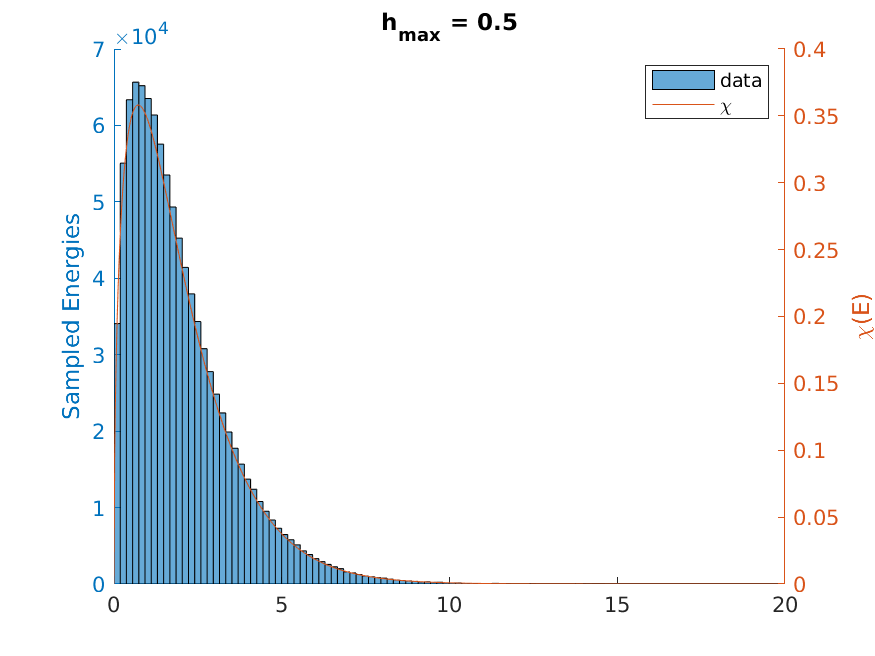
\includegraphics[width=0.8\textwidth]{standard_rejection_hmax}
          \caption{Sampling with standard rejection and reduced efficiency.}
          \label{fig:standard_rejection_hmax}
        \end{figure}

      \item Develop a two region partioned rejection scheme for sampling the
        fisiosn neutron spectrum. Determine the maximum efficiency that can be
        obtained with the two region scheme. Show that the partitioned scheme
        generates energies according to the fission neutron spectrum. Verify
        numerically the efficiency of the partitioned scheme.

        A partitioned scheme specifies some point $x_1$. Then, standard
        rejection sampling is performed in $[a,x_1]$ and $[x_1,b]$ with values
        $h_{max1}$ and $h_{max2}$. The key lies in determining the point $x_1$
        to maximize the efficiency of the scheme. The following are quantities
        necessary for the optimization of this efficiency. For this
        implementation, $E_{max} = 20 \text{MeV}$. 
        \begin{align}
          h_{max1} &= \max_{E \in [0,x_1]} \chi(E) \\
          h_{max2} &= \max_{E \in [x_1,E_{max}]} \chi(E) \\
          H_1 &= \int_0^{x_1} \chi(E) \; dE \\
          H_2 &= \int_{x_1}^{E_{max}} \chi(E) \; dE \\
          \epsilon_1 &= \frac{H_1}{h_{max1} x_1} \\
          \epsilon_2 &= \frac{H_2}{h_{max2} (E_{max} - x_1)} \\
          \epsilon &= \frac{1}{\frac{H_1}{\epsilon_1} + \frac{H_2}{\epsilon_2}}
        \end{align}
        The above equations can be solved for a given $x_1$ and be optimized for
        maximum efficiency. For this method, a binary search was used resulting
        in $x_1 = 5.25$ and $\epsilon = 0.426577$. Other quantities can then be
        precalculated and stored as runtime constants in a monte carlo code. 

        Numerically, it can be shown that this optimized partition method also
        results in sampling from the fission spectrum as shown in Figure
        \ref{fig:partition_scheme}. The numeric efficiency scheme for $10^6$
        samples was 0.427921.

        \begin{figure}
          \centering
          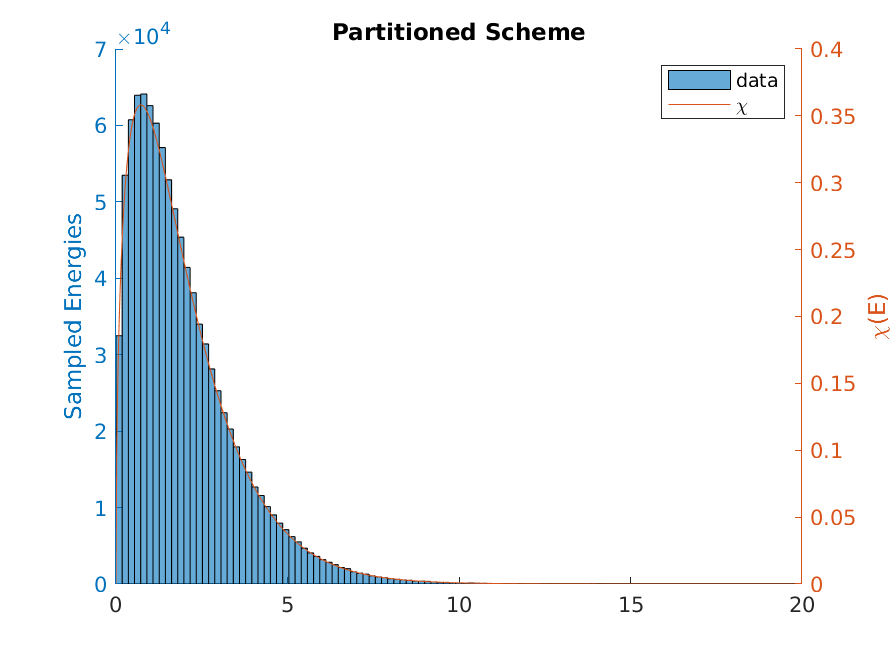
\includegraphics[width=0.8\textwidth]{partition_scheme}
          \caption{Sampling with optimized partition rejection.}
          \label{fig:partition_scheme}
        \end{figure}

      \item 
        \label{part:standard}
        Use the standard rejection scheme to determine both the average
        number of neutrons per fission and the average fissions neutron
        energy. Compare to the ``analytic'' result.
        
        Using the standard rejection scheme, the average number of neutrons
        per fission and the average fission neutron energy were determined.
        Results are presented in Table \ref{tab:standard}. The mean and 
        uncertainty are presented a sa function of the number of samples in 
        Figure \ref{fig:standard_energy_mean}, Figure 
        \ref{fig:standard_energy_variance}, Figure \ref{fig:standard_nu_mean},
        and Figure \ref{fig:standard_nu_variance}. 

        \begin{table}
          \caption{Standard Rejection Results. N = $10^4$.}
          \label{tab:standard}
          \begin{center}
          \begin{tabular}
            & Mean & Variance & Uncertainty \\
            \midrule
            Energy & 1.998684&  2.417327&  0.000242\\
            $\nu$  & 2.656156&  0.050936&  0.000005
          \end{tabular}
          \end{center}
        \end{table}

        \begin{figure}
          \centering
          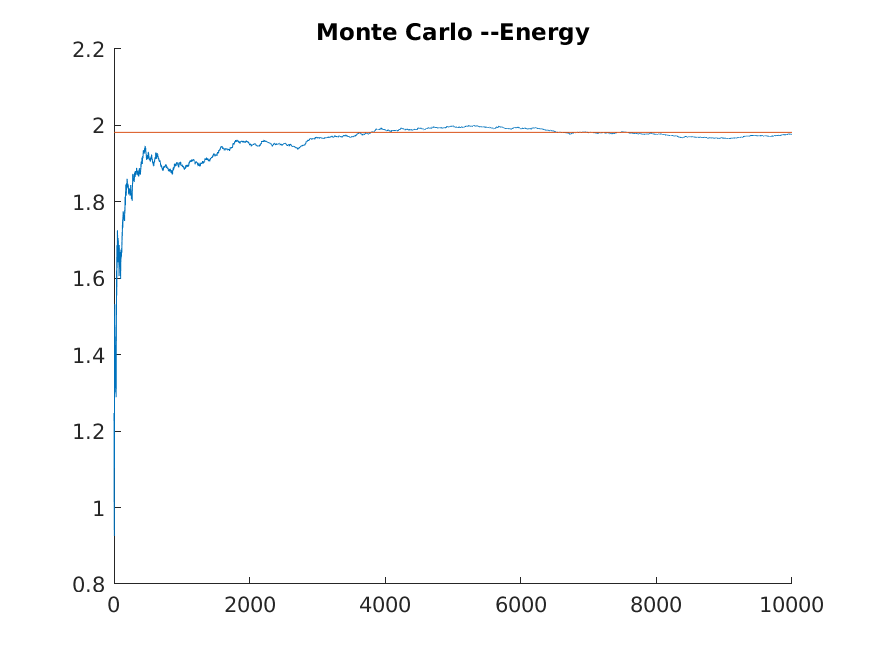
\includegraphics[width=0.8\textwidth]{standard_energy_mean}
          \caption{Standard Sampling. Energy Mean.}
          \label{fig:partition_scheme}
        \end{figure}

        \begin{figure}
          \centering
          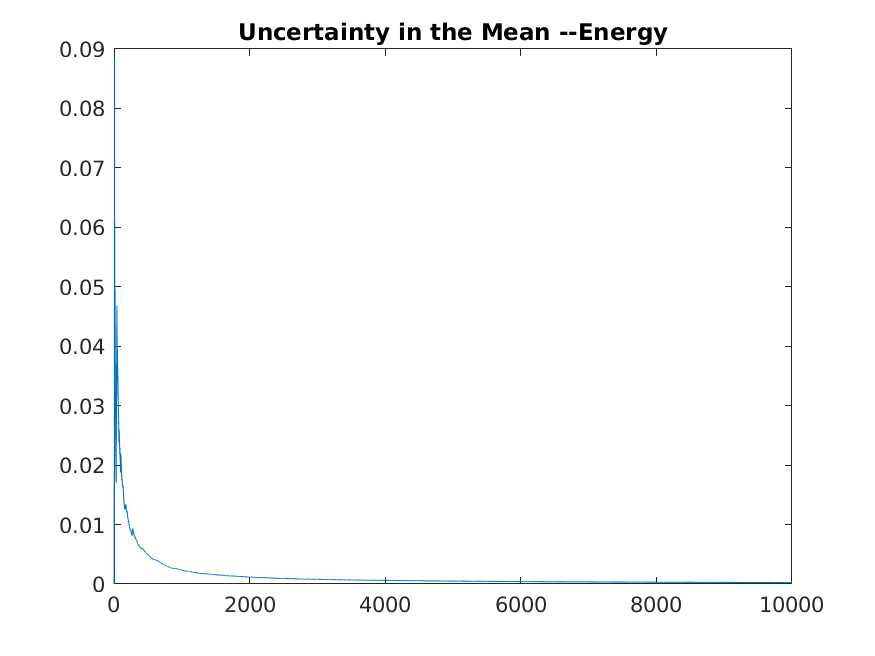
\includegraphics[width=0.8\textwidth]{standard_energy_uncertainty}
          \caption{Standard Sampling. Energy Uncertainty.}
          \label{fig:standard_energy_uncertainty}
        \end{figure}

        
        \begin{figure}
          \centering
          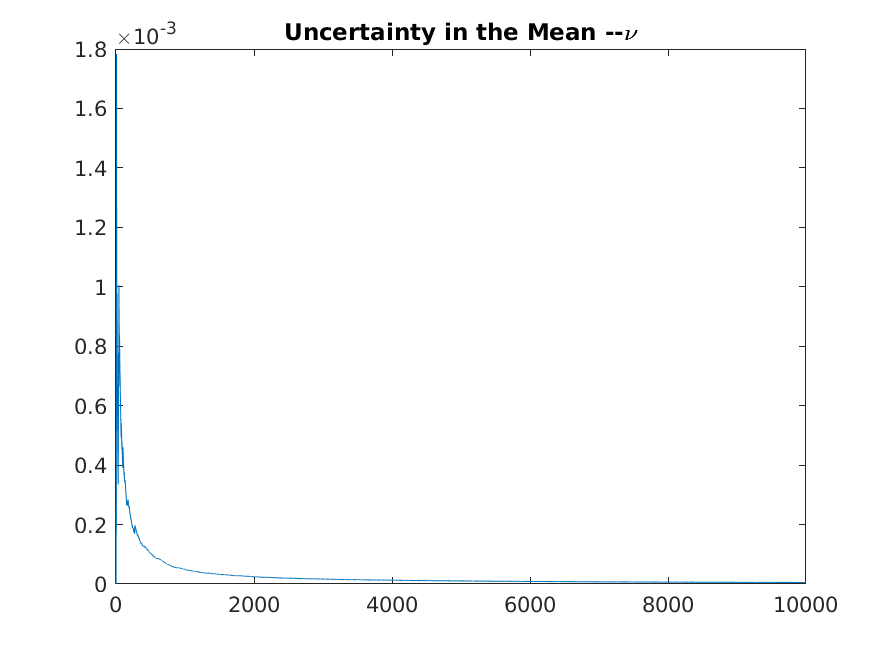
\includegraphics[width=0.8\textwidth]{standard_nu_uncertainty}
          \caption{Standard Sampling. $\nu$ Uncertainty.}
          \label{fig:standard_nu_uncertainty}
        \end{figure}

        \begin{figure}
          \centering
          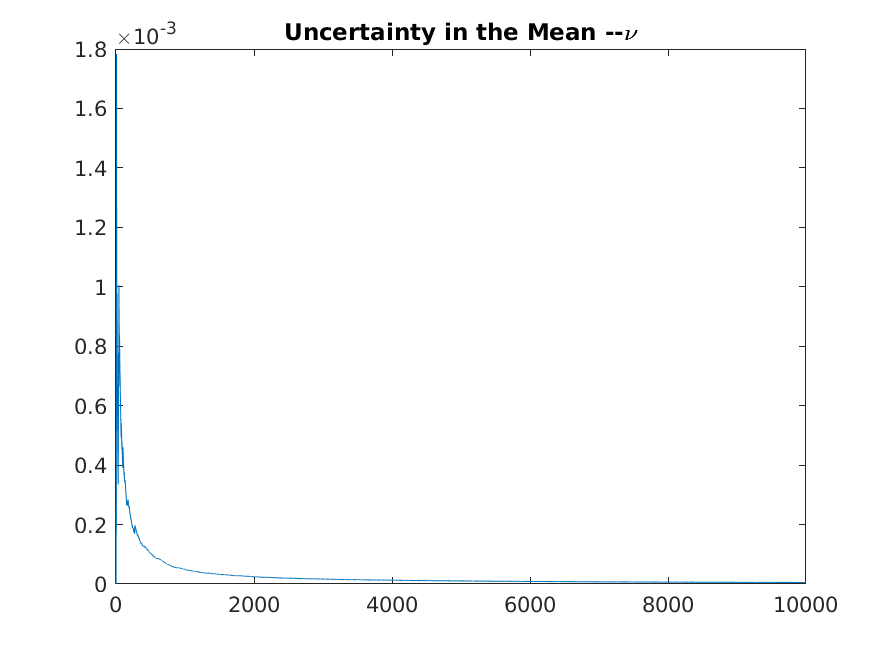
\includegraphics[width=0.8\textwidth]{standard_nu_uncertainty}
          \caption{Standard Sampling. $\nu$ Uncertainty.}
          \label{fig:standard_nu_uncertainty}
        \end{figure}

      \item Repeat part \ref{part:standard} using maximum efficiency scheme.
      
        Using the partition rejection scheme, with maximum efficiency, 
        the average number of neutrons per fission and the average fission 
        neutron energy were determined. This is expected to agree to the 
        standard scheme to within statistical error as the two schemes are 
        equivalent. Results are presented in Table \ref{tab:partition}. The 
        mean and uncertainty are presented as a function of the number 
        of samples in Figure \ref{fig:partition_energy_mean}, Figure 
        \ref{fig:partition_energy_variance}, Figure \ref{fig:partition_nu_mean},
        and Figure \ref{fig:partition _nu_variance}. 
        
        \begin{table}
          \caption{Partition Rejection Results. N = $10^4$.}
          \label{tab:partition}
          \begin{center}
          \begin{tabular}
            & Mean & Variance & Uncertainty \\
            \midrule
            Energy & 1.985709&  2.457664&  0.000246\\
            $\nu$  & 2.654359&  0.051806&  0.000005
          \end{tabular}
          \end{center}
        \end{table}

        \begin{figure}
          \centering
          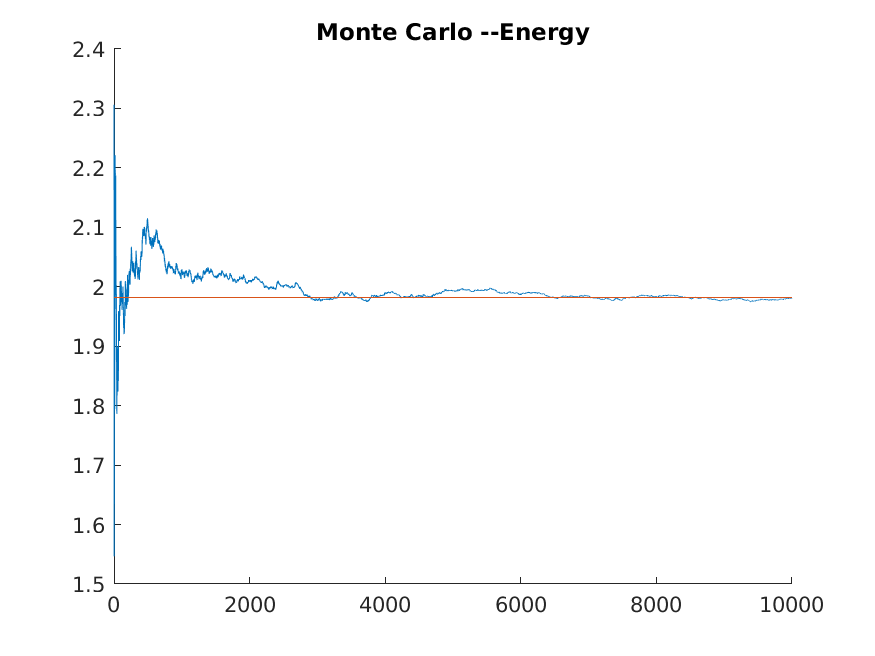
\includegraphics[width=0.8\textwidth]{partition_energy_mean}
          \caption{Partition Sampling. Energy Mean.}
          \label{fig:partition_scheme}
        \end{figure}

        \begin{figure}
          \centering
          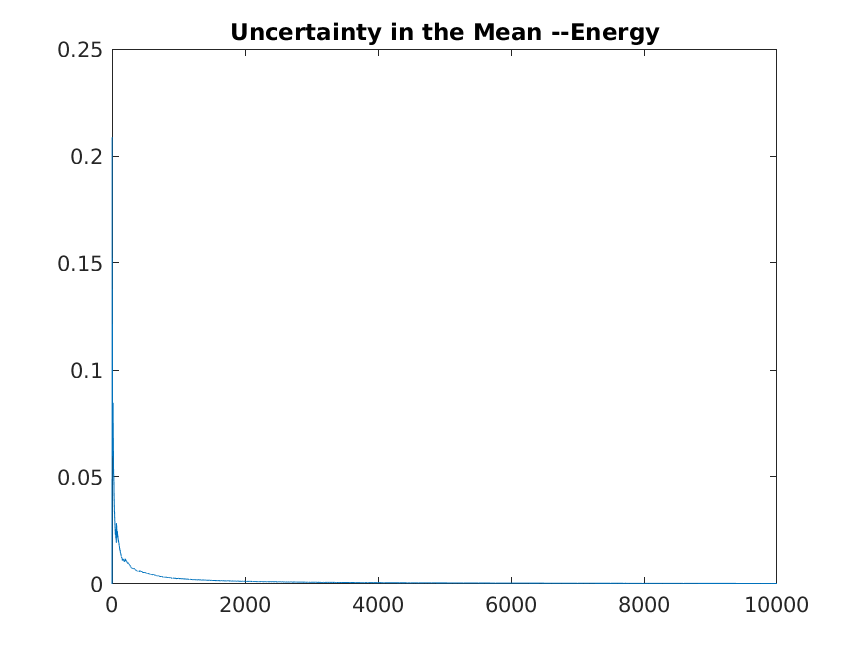
\includegraphics[width=0.8\textwidth]{partition_energy_uncertainty}
          \caption{Partition Sampling. Energy Uncertainty.}
          \label{fig:partition_energy_uncertainty}
        \end{figure}

        
        \begin{figure}
          \centering
          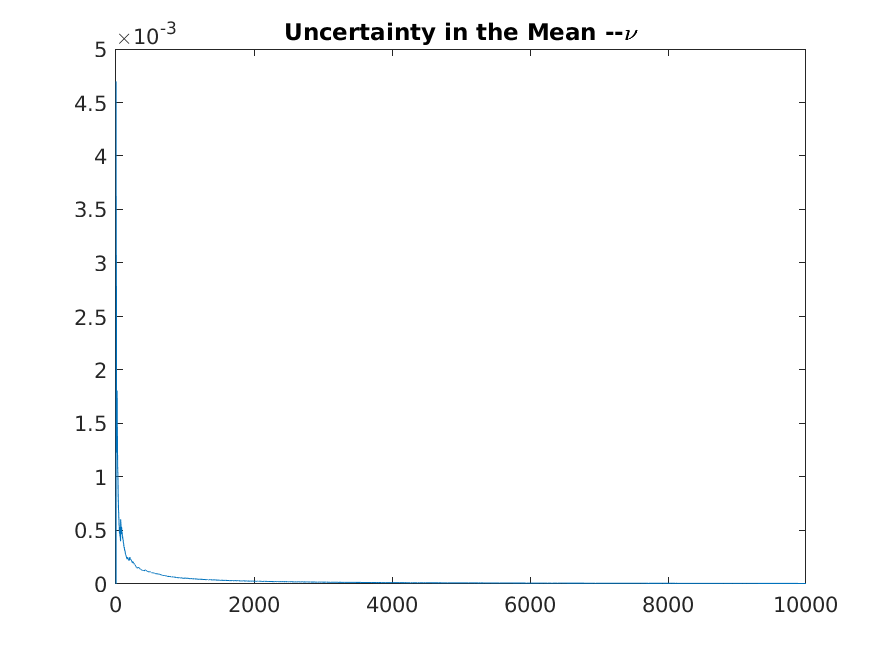
\includegraphics[width=0.8\textwidth]{partition_nu_uncertainty}
          \caption{Partition Sampling. $\nu$ Uncertainty.}
          \label{fig:partition_nu_uncertainty}
        \end{figure}

        \begin{figure}
          \centering
          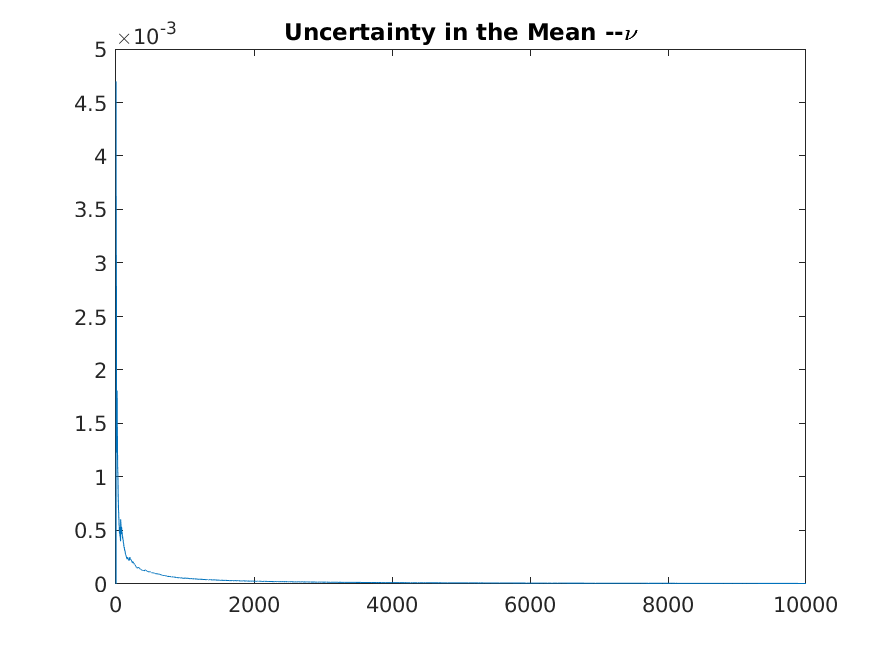
\includegraphics[width=0.8\textwidth]{partition_nu_uncertainty}
          \caption{Partition Sampling. $\nu$ Uncertainty.}
          \label{fig:partition_nu_uncertainty}
        \end{figure}
    \end{enumerate}
\end{enumerate}

\end{document}
